\documentclass[12pt]{article}
\usepackage[margin=1in]{geometry}
\usepackage{amsmath,amssymb,amsthm,booktabs,graphicx,natbib,microtype,array}
\newtheorem{theorem}{Theorem}
\newtheorem{corollary}[theorem]{Corollary}
\newtheorem{proposition}[theorem]{Proposition}
\newtheorem{remark}[theorem]{Remark}
\title{Ten-Layer Controlled-Viability Review\\\large RH-130--RH-139 and a Revised Minimal Directional Frontier}
\author{Prime Dynamics Theory Program}
\date{July 2026}

\begin{document}
\maketitle

\begin{abstract}
We review RH-130--RH-139 as one proof system.  The ten layers remove the
positive-Gram floor, treat singular support, derive a model-generated moving
frame, expose target-metric amplification, solve the orthogonal metric
minimax problem, replace stationary fixed-floor optimization by a
finite-horizon control envelope, and close the frozen finite chain with
outward Loewner guards.  The finite progression is substantial: the initial
floor-free transfer has zero positive complete chains, the Euclidean polar
gauge has only 51/216 contractive recurrent transitions, metric balancing
recovers 183/216, finite-horizon control certifies 328/330 transitions and
28/30 chains, and outward composition retains all 28 positive chains.

The main theoretical conclusion is a weaker and more accurate all-level
frontier.  Let $y_n$ be any validated controlled upper for the squared
relative tail and let
$a_n=\sqrt{\lambda_{\min}(G_n)/\lambda_{\max}(G_n)}$.  If
\[
 \limsup_{n\to\infty}y_n\leq \bar y<1,
 \qquad
 \liminf_{n\to\infty}a_n\geq a_*>0,
\]
then the directional candidates obey
\[
 \liminf_{n\to\infty}B_n
 \geq(1-\sqrt{\bar y})^4a_*>0.
\]
This theorem does not require a subunit affine coefficient at every step;
isolated expanding transitions may be crossed by a state-dependent viability
policy.  The two hypotheses are separately sharp within the directional
candidate architecture: allowing $y_n\to1$ or $a_n\to0$ destroys every
positive universal floor.

Thus the exact-matrix mathematical frontier is reduced to two packets:
eventual uniform controlled-tail viability and a positive normalized-base
liminf.  A validated model route additionally needs exact or interval source
enclosure; independently assembled routes also need all-level outward radii.
All nine upstream archives and claim boundaries pass an automated review.
None of the three missing all-level packets is proved here.
\end{abstract}

\section{What changed over ten layers}
RH-129 identified an all-level subunit affine Rayleigh recurrence and a
positive normalized-base liminf as the directional frontier.  RH-130--RH-138
reopened the first packet from the physical packet construction rather than
from post-hoc regularized Gramians.  Three changes proved decisive.

First, singularity is structural rather than numerical.  RH-130 and RH-131
show that the recent action may have zero tail rank followed by rank birth,
so the correct quotient lives on the supported subspace.  Second, the raw
memory coefficient is strongly contractive but the recent-Gram metric is not:
RH-134 gives a raw factor below $0.003914$, whereas RH-135 finds a polar-gauge
relative base as large as $3.03\times10^7$.  Third, long-run contractivity is
not the same as finite viability.  RH-136 proves 33 transitions are
noncontractive for every orthogonal gauge, but RH-137 crosses 31 of them
safely because their incoming certified state is small.

This last observation changes the proof obligation.  The route does not need
$\rho_n<1$ at every level.  It needs a controlled state that eventually stays
a uniform distance below the support wall.  This is a viability condition in
the standard control-theoretic sense \citep{Aubin1991}, specialized here to a
scalar order-preserving envelope.

\section{Controlled viability replaces per-step contraction}
At level $n$, let $x_n=\gamma_n^2$ be the actual squared relative tail.  A
finite family of packet gauges gives monotone Young envelopes
\[
 F_{n,c}(y)=q_{n,c}+
 \left(\sqrt{A_{n,c}y}+\sqrt{B_{n,c}}\right)^2,
 \qquad c\in\mathcal C_n.
\]
If $y_n\geq x_n$, define the controlled upper
\begin{equation}\label{eq:control}
 y_{n+1}=\inf_{c\in\mathcal C_n}F_{n,c}(y_n).
\end{equation}
RH-137 proves that for a finite candidate family this greedy choice minimizes
every later finite-horizon envelope.  RH-138 shows how two outward residuals
can validate each chosen transition from rounded matrices and radii.

Let
\[
 a_n=\frac{\sqrt{\det G_n}}{L_n^4C_n}
 =\sqrt{\frac{\lambda_{\min}(G_n)}
 {\lambda_{\max}(G_n)}}
\]
be the normalized directional base.  The candidate lower is
\begin{equation}\label{eq:candidate}
 B_n=(1-\sqrt{x_n})_+^4a_n.
\end{equation}

\begin{theorem}[Eventual controlled-viability support]\label{thm:viability}
Suppose $x_n\leq y_n$ eventually and
\[
 \limsup_{n\to\infty}y_n\leq\bar y<1,
 \qquad
 \liminf_{n\to\infty}a_n\geq a_*>0.
\]
Then
\[
 \liminf_{n\to\infty}B_n
 \geq(1-\sqrt{\bar y})^4a_*>0.
\]
Consequently, every fixed threshold strictly below this floor is eventually
supported by the directional candidate.
\end{theorem}

\begin{proof}
Since $x_n\leq y_n$ and $z\mapsto(1-\sqrt z)_+^4$ is decreasing,
\[
 B_n\geq(1-\sqrt{y_n})_+^4a_n.
\]
For every $\varepsilon>0$, eventually
$y_n\leq\bar y+\varepsilon<1$ and $a_n\geq a_*-\varepsilon$.
Taking the lower limit and then $\varepsilon\downarrow0$ proves the formula.
\end{proof}

The theorem strictly weakens the RH-128 route.  A contractive affine
recurrence is one sufficient method for constructing the required tube, but
it is not part of the conclusion and need not hold at isolated steps.  For
example, $F(y)=My$ has coefficient $M>1$ yet crosses safely whenever
$y<1/M$.  What matters is the global controlled trajectory, not the sign of
one local logarithmic multiplier.

\begin{proposition}[Architecture-sharp frontier]\label{prop:sharp}
Within the candidate formula \eqref{eq:candidate}, neither the strict
uniform tail gap nor the positive base liminf can be removed from a universal
positive eventual lower.
\end{proposition}

\begin{proof}
For the tail-gap obstruction, take
$y_n=x_n=(1-1/n)^2$ and $a_n=1$.  Then $y_n\uparrow1$ and
$B_n=n^{-4}\to0$.  For the base obstruction, take $x_n=y_n=0$ and
$a_n=1/n$.  Again $B_n\to0$.  Both examples satisfy the other packet in its
strongest form.
\end{proof}

This is an architecture-relative necessity statement, not a claim that every
possible proof of a broader theorem must use these variables.

\section{Layer-by-layer audit}
Table~\ref{tab:layers} records the logical role of each paper.  ``Mixed''
means that a constructive theorem and a sharp obstruction are equally central.

\begin{table}[t]
\centering
\scriptsize
\renewcommand{\arraystretch}{1.12}
\begin{tabular}{cclp{6.1cm}}
\toprule
RH & type & exact contribution & finite consequence or obstruction \\
\midrule
130 & mixed & floor-free semidefinite minimax & 118/120 positive states, but 0/24 complete chains; 24 rank births \\
131 & constructive & support quotient and pseudovolume & kernel leakage exactly characterizes infinite relative quotients \\
132 & constructive & canonical partial-isometry forcing & trace-minimal forcing; 22/24 birth strengths subunit \\
133 & mixed & dyadic packet gauge & 65 versus 67 positive transfers; angle-only bounds fail sharply \\
134 & constructive & exact memory/birth recurrence & 330/330 identities and Loewner bounds; birth dominates forcing \\
135 & mixed & sharp relative affine coefficients & polar gauge contractive on only 51/216 recurrent steps \\
136 & constructive & orthogonal metric minimax & 183/216 possible and recovered; 33 universal orthogonal walls \\
137 & constructive & pointwise Young viability control & 31/33 walls crossed; 328/330 safe steps and 28/30 chains \\
138 & constructive & outward residual/base composition & 330/330 residual pairs; 28 outward-positive chains; precision gate \\
139 & synthesis & controlled-viability frontier & per-step contraction removed; two sharp remaining mathematical packets \\
\bottomrule
\end{tabular}
\caption{The RH-130--RH-139 proof stack.}
\label{tab:layers}
\end{table}

The automated review reads every upstream summary and archive-verification
record, hashes the nine summaries, and inspects the explicit program
boundaries.  All nine archives verify and no Stage A, Hilbert--Polya, or RH
flag is asserted.  A 4,096-instance scalar audit of
Theorem~\ref{thm:viability} has zero floor failures.  The two sharp witness
families are also archived.

\begin{figure}[t]
\centering
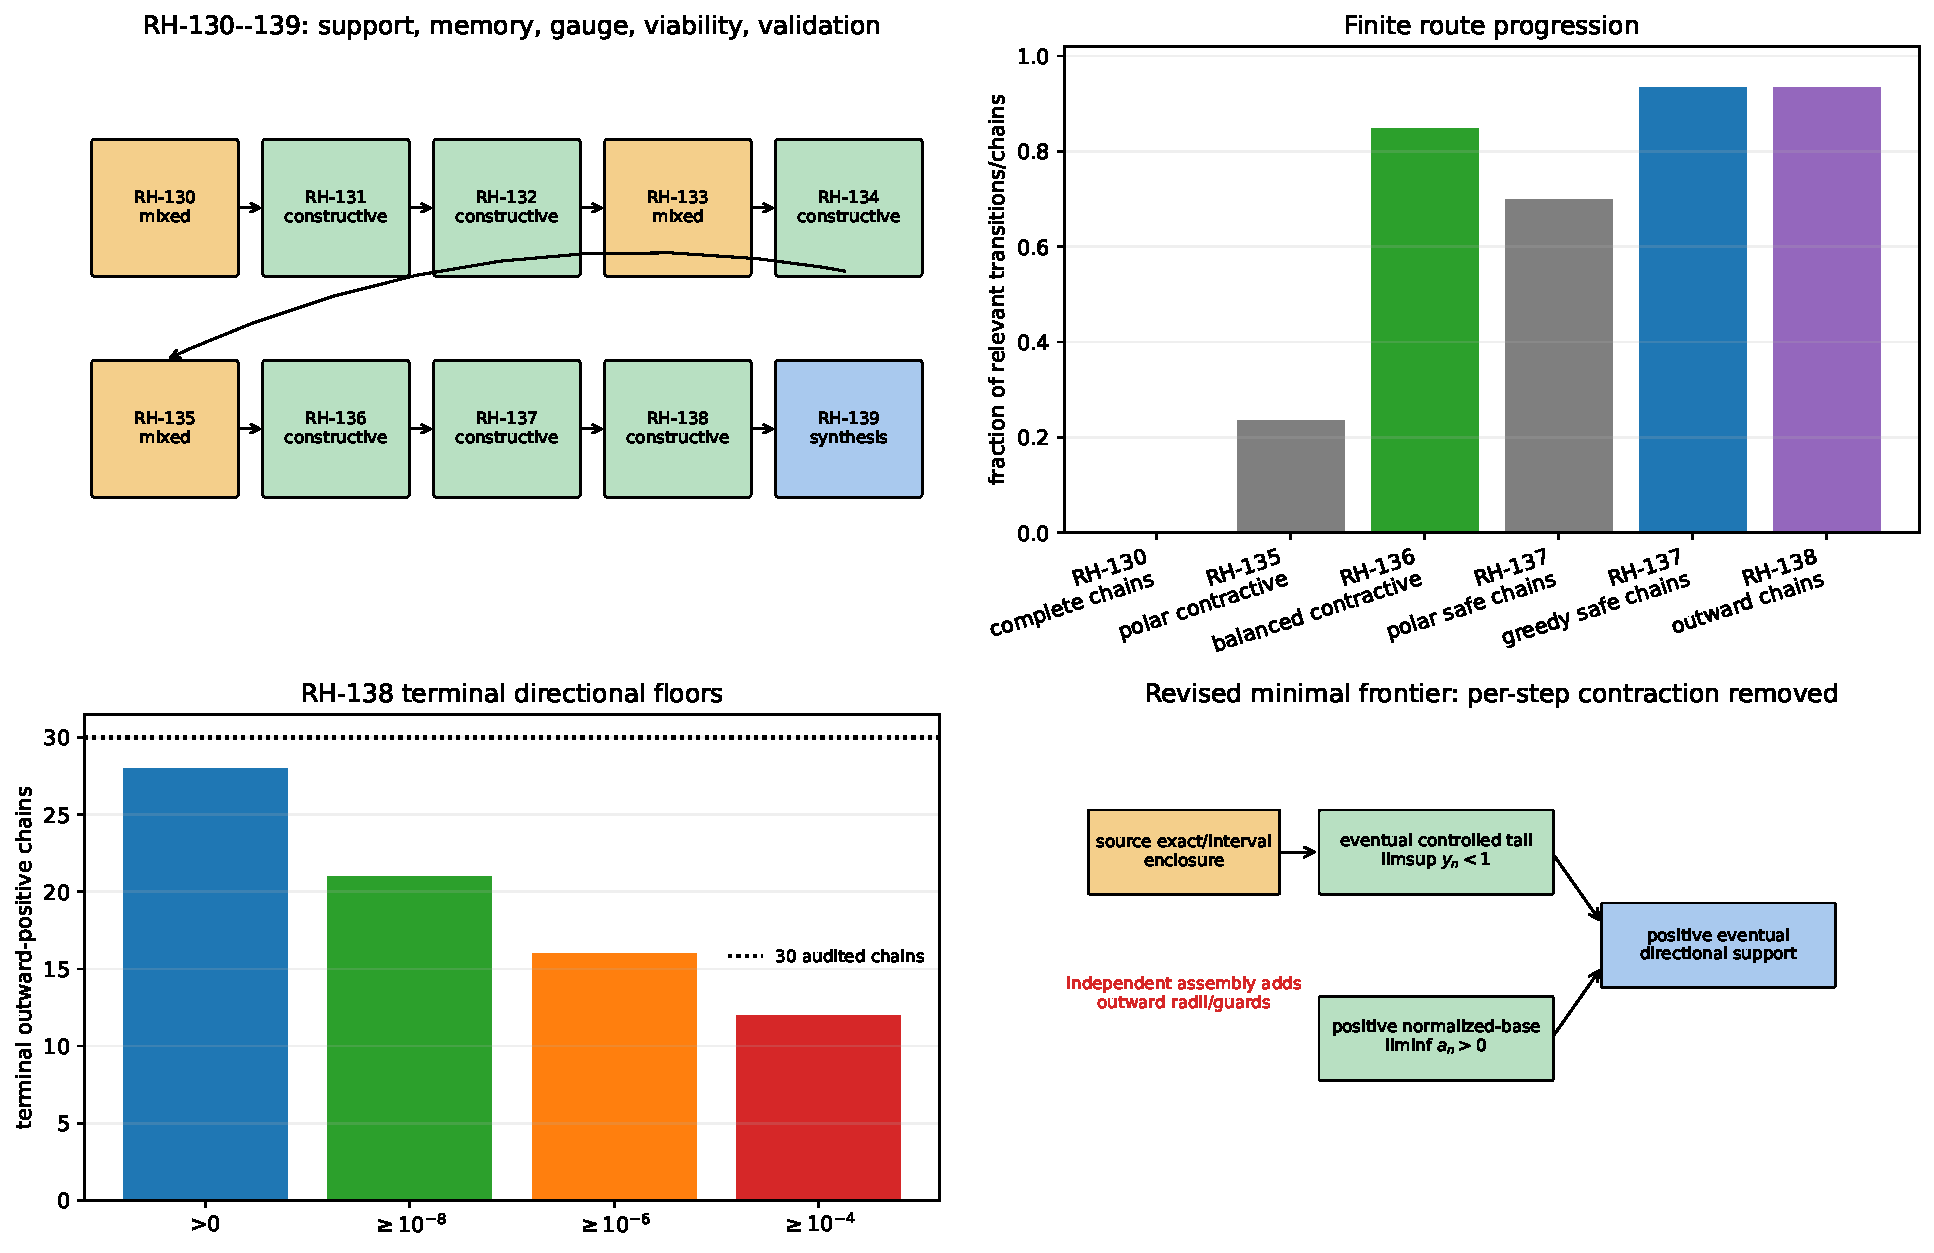
\includegraphics[width=\textwidth]{figures/ten_layer_controlled_viability_review.pdf}
\caption{The ten-layer dependency path, finite progression, terminal
directional floors, and the revised minimal frontier.}
\label{fig:review}
\end{figure}

\section{What the finite result now says}
The frozen packet family has moved from no complete floor-free chains to 28
outward-positive chains.  This improvement is not produced by one optimistic
regularization.  It comes from four identifiable corrections:
supported-subspace quotients, the exact memory recursion, metric-aware gauge
selection, and state-dependent finite-horizon optimization.  RH-138 then
shows that 40-decimal independent rounding and explicit norm radii preserve
the result with negligible outward padding.

The terminal directional lowers of the 28 positive chains range above
$10^{-10}$; 21 exceed $10^{-8}$, 16 exceed $10^{-6}$, and 12 exceed
$10^{-4}$.  The two failed chains are coarse left-channel cases whose new
boundary term is already $9.40589>1$ relative to the target Gram.  They do not
show that an eventual-start theorem is impossible: an asymptotic route may
begin after finitely many coarse events.  They do show that a certificate
starting from the present rank-four/depth-eight initialization cannot retain
all 30 chains.

The finite precision result has a similarly exact boundary.  Twenty decimal
digits suffice to keep every archived normalized base positive under a norm
ball, whereas fp64 loses ten weak coarse directions.  By the RH-138
norm-ball barrier, these ten losses cannot be repaired by a cleverer
eigenvalue inequality without adding information \citep{Bhatia1997,
HornJohnson1991,Moore1966}.

\section{Revised minimal frontier}
For exact all-level matrices, Theorem~\ref{thm:viability} and
Proposition~\ref{prop:sharp} leave the inclusion-minimal frontier
\[
 \boxed{P_V:\ \limsup y_n<1},
 \qquad
 \boxed{P_B:\ \liminf a_n>0}.
\]
Here $P_V$ may be obtained by block control, resets, delayed start, occasional
metric expansion followed by strong contraction, or another monotone policy.
It is strictly weaker than requiring every affine base or every optimized
$\rho_n$ to be subunit.

To connect these exact-matrix packets to the intended model, add
\[
 \boxed{P_E:\ \text{exact or interval source-to-packet enclosure}}.
\]
If source, tail, forcing, and target matrices are assembled independently,
the RH-127/RH-138 logic additionally requires
\[
 \boxed{P_O:\ \text{all-level outward radii and residual guards}}.
\]
Thus the two validated routes are
\[
 \{P_V,P_B,P_E\}\quad\text{(common assembly)},
 \qquad
 \{P_V,P_B,P_E,P_O\}\quad\text{(independent assembly)}.
\]
The current work supplies finite evidence and exact algebra for every box,
but proves none of $P_V,P_B,P_E$ all levels.

\section{Next research block and claim boundary}
The next block should be narrower than the preceding maze exploration.
First, intervalize the source snapshots and packet/frame construction so that
RH-138 validates the intended model rather than only a frozen reference.
Second, search for an all-level block or reset theorem for the controlled map
\eqref{eq:control}; the correct target is a uniform viability tube, not
per-step contraction.  Third, attack the weakest-direction base $a_n$ on the
same correlated assembly path, avoiding the separate volume/capacity loss
identified in RH-124.  A delayed-start analysis should determine whether the
two coarse birth failures are irrelevant to an eventual statement.

Only after these packets close would the directional Stage A branch have an
all-level foundation.  RH-139 does not prove the controlled tail gap, the
positive base liminf, source-model interval enclosure, all-level outward
radii, uniform Stage A, a Hilbert--Polya operator, zeta-zero identification,
or the Riemann Hypothesis.

\bibliographystyle{plainnat}
\bibliography{references}
\end{document}
